\documentclass[11pt,xcolor=svgnames]{beamer}
\usepackage{dsfont,natbib,setspace,changepage,multirow}
\mode<presentation>

% replaces beamer foot with simple page number
\setbeamertemplate{navigation symbols}{}
\setbeamerfont{frametitle}{series=\bfseries,size=\normalsize}
\setbeamercolor{frametitle}{fg=Black}

\setbeamertemplate{footline}{
   \raisebox{5pt}{\makebox[\paperwidth]{\hfill\makebox[20pt]{\color{gray}\scriptsize\insertframenumber}}}}

\usepackage{algorithm}
\usepackage{algorithmic}

% colors
\newcommand{\theme}{\color{DarkBlue}}
\newcommand{\bk}{\color{black}}
\newcommand{\rd}{\color{red}}
\newcommand{\fg}{\color{ForestGreen}}
\newcommand{\bl}{\color{blue}}
\newcommand{\gr}{\color{black!50}}
\newcommand{\sg}{\color{DarkSlateGray}}
\newcommand{\nv}{\color{Navy}}
\setbeamercolor{itemize item}{fg=gray}

% common math markups
\newcommand{\bs}[1]{\boldsymbol{#1}}
\newcommand{\mc}[1]{\mathcal{#1}}
\newcommand{\mr}[1]{\mathrm{#1}}
\newcommand{\bm}[1]{\mathbf{#1}}
\newcommand{\ds}[1]{\mathds{#1}}
\newcommand{\indep}{\perp\!\!\!\perp}
\def\plus{\texttt{+}}
\def\minus{\texttt{-}}

% spacing and style shorthand
\setstretch{1.1}

\begin{document}

\setcounter{page}{0}
{ \usebackgroundtemplate{
\includegraphics[height=\paperheight]{phoenix}}
\begin{frame}[plain]
\begin{center}

{\bf \LARGE \theme }

{\bf \Large  Big Data and Bayesian Nonparametrics}

\vskip 2cm
Matt Taddy,  Chicago Booth


\vskip .25cm
{\texttt{faculty.chicagobooth.edu/matt.taddy/research}}

\end{center}
\end{frame} }


\begin{frame}

{\bf Big Data}

\vskip .25cm

\vskip .25cm
{\nv The sample sizes are enormous.}
\begin{itemize}
\item We'll see 21 and 200 million today.  
\item Data can't fit in memory, or even storage, on a single machine.
%\item Our familiar MCMC algorithms take too long.
\end{itemize}


\vskip .25cm
{\nv The data are super weird.  }
\begin{itemize}
\item Internet transaction data distributions have a big spike at zero and spikes at other discrete values (e.g., 1 or \$99).
\item Big tails (e.g., \$12 mil/month eBay user spend) that matter.
\item The potential feature space is unmanageably large.
\item We cannot  write down or measure believable models.
\end{itemize}

\vskip .5cm\theme
Both `Big' and `Strange' beg for nonparametrics.

\end{frame}

\begin{frame}

{\bf Bayesian nonparametrics}

\vskip .5cm
In usual BNP you {\it model} a complex generative process with flexible priors, then apply that model directly in prediction and inference.

\vskip .25cm
~~~~~~~e.g.,~~~~ $y = f(\bm{x}) + \varepsilon$ ~~~%{\gr additive error semiparametric regression.}
or ~~~ $f(y|\bm{x}) = f(\bm{x},y)/f(\bm{x})$ %{\gr implied conditionals / kernel regression}

\vskip .25cm
`Flexibility' comes from a huge number of variables,
\[
\text{e.g.,}~~~~~ f(\bm{z}) = \sum_{k=1}^{{\theme \infty}} \omega_k \mr{N}(\bm{z};~\bs{\mu}_k,\bs{\Sigma}_k),
\]
and learning requires integration over uncertainty on nuisance parameters, e.g., $k_i$  component membership for observation $\bm{z}_i$.

\vskip .5cm 
For years this integration was done via MCMC. But these algorithms did not scale for big data.   {\theme Can we do scalable BNP?}


\end{frame}

\begin{frame}

{\bf Classical distribution-free nonparametrics}

\vskip .5cm
Frequentists are great at finding simple procedures {\gr\small (e.g. $[\bm{X}'\bm{X}]^{-1}\bm{X}'y$)\!\!} and  describing how they work under a variety of possible true DGP.

\hfill{\nv (~DGP = Data Generating Process~)}

\vskip .5cm
This is `distribution free' nonparametrics.

\vskip .15cm
1: Find some statistic that is useful regardless of DGP.

\vskip .15cm
2: Derive the distribution for this stat under minimal assumptions.

\vskip .5cm
Practitioners apply the simple stat and feel happy that it will work.

% \vskip .2cm
% No need to re-model the underlying DGP each time, and you \\don't need to have a PhD in  Statistics to apply the ideas.

\end{frame}

\begin{frame}

{\bf Distribution-free Bayesian nonparametrics}

\vskip .5cm
{Find some {\it statistic of the DGP} that you care about:}
\vskip .1cm
\begin{itemize}
\item derive from first principles, e.g. moment conditions
\item {\it an algorithm} that we know works, e.g. CART
\item think about geometric projections, e.g. OLS
\end{itemize}
\vskip .1cm
Call this statistic $\bs{\theta}(g)$ where $g(\bm{z})$ is the DGP (e.g., for $\bm{z} = [\bm{x},y]$).

\vskip .5cm
Then you write down a flexible  model for the DGP $g$, and study properties of the posterior on $\bs{\theta}(g)$ induced by the posterior over $g$.

\end{frame}

\begin{frame}

{\bf A flexible model for the DGP}

\vskip .5cm
Say $\bm{z} = [\bm{x},y]$ is a single {\it independent} data point.

\vskip .25cm Each data point assumes one of a {\it finite} number of possible values, $[\bs{\zeta}_1 \ldots \bs{\zeta}_L]$, with probabilities proportional to $[\bs{\theta}_1 \ldots \bs{\theta}_L]$.
\begin{equation*}
g(\bm{z}) = \frac{1}{|\bs{\theta}|}\sum_{l=1}^L \theta_l \ds{1}_{[\bm{z} =
\bs{\zeta}_l]}\end{equation*}

We complete specification with a conjugate prior on the weights:
\[\frac{\bs{\theta}}{|\bs{\theta}|} \sim \mr{Dir}(a) \propto \frac{1}{|\bs{\theta}|^{L(a-1)}}\prod_l \theta_l^{a-1}~~\text{where}~~a,\theta_l >0.
\]
%The support is treated as fixed.

%\vskip .25cm
This is the Dirichlet-multinomial sampling model {\gr (Ferguson 1973)}.  

\end{frame}

\begin{frame}

Now you've observed some data, say $\bm{Z} = \{\bm{z}_1 \ldots \bm{z}_n\}$.\\
{\gr (say every $\bm{z}_i = [\bm{x}_i,y_i]$ is unique)}.

\vskip .25cm
The posterior over weights has $\theta_l \stackrel{ind}{\sim} \mr{Exp}\left(a+\ds{1}_{[\bs{\zeta}_l \in \bm{Z}]}\right)$. 

\vskip .5cm
{\bf A convenient limiting case}

\vskip .25cm
$a \to 0$ leads to $\mr{p}(\theta_l = 0) = 1$ for $\bs{\zeta}_l \notin \bm{Z}$.

\vskip .2cm
In this case, we can focus on only the {\it observed support} and write the posterior for our DGP
\[
g(\bm{z}) = \tfrac{1}{|\bs{\theta}|}
\sum_{i=1}^n \theta_i \ds{1}{[\bm{z} =
\bm{z}_i]},~~~\theta_i \stackrel{iid}{\sim} \mr{Exp}(1).
\]

\hfill
{This is just the Bayesian bootstrap. \gr (Rubin 1981)}

\end{frame}


% \begin{frame}

% \vskip .25cm
% Recall your early stats: {\theme the sampling distribution.}

% \vskip .1cm
% Imagine getting multiple datasets of size $n$ from the population.

% \vskip .1cm
% The {\it sampling distribution} of an estimator $\hat \beta$\\ is
% the histogram of your estimates for each dataset.


% \vskip .25cm
% 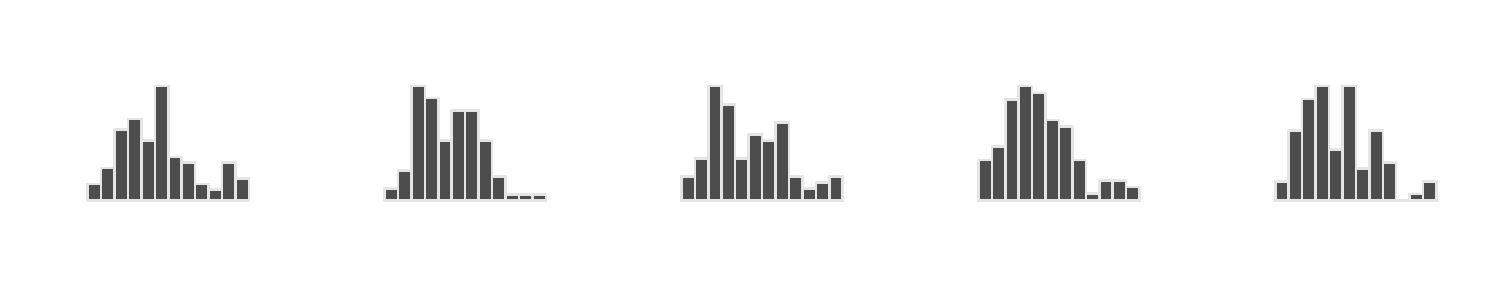
\includegraphics[width=4.2in]{graphs/bs_boothist}

% \vskip -.2cm
% $
% ~\begin{array}{c}\downarrow\\
%     \hat\beta_1\\
%     ~~\searrow
% \end{array}
% $
% \hskip 1.1cm
% $
% \begin{array}{c}\downarrow\\
%     \hat\beta_2\\
%     ~~\searrow
% \end{array}
% $
% \hskip 1.1cm
% $
% \begin{array}{c}\downarrow\\
%     \hat\beta_3\\
%     \downarrow
% \end{array}
% $
% \hskip 1.1cm
% $
% \begin{array}{c}\downarrow\\
%     \hat\beta_4\\
%     \swarrow~~
% \end{array}
% $
% \hskip 1.1cm
% $
% \begin{array}{c}\downarrow\\
%     \hat\beta_5\\
%     \swarrow~~
% \end{array}
% $

% \begin{center}
% 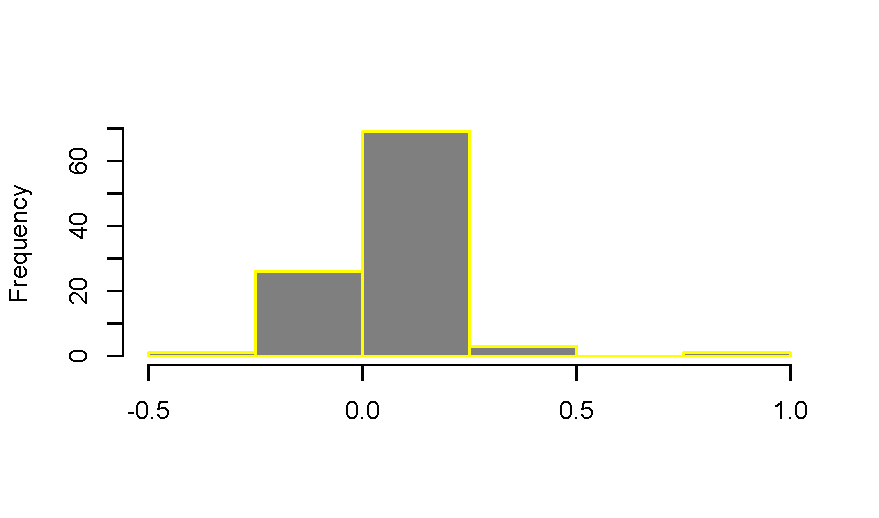
\includegraphics[width=2.25in]{graphs/boothist}
% \end{center}
 

% \vskip -.5cm
% \end{frame}

% \begin{frame}


% {\bf \theme The Bootstrap:} resample your data {\it with replacement} \\
% ~~~~~~~~~~~~~~~~~~ and calculate  some statistic of interest.  

% \vskip .1cm {\it \gr With-Replacement: each draw is put back in the `bucket', so it is possible to sample the same
% observation multiple times.  }

% \vskip .5cm
% To raise oneself up by bootstraps...  
% {\gr (Try it; it doesn't work).}

% \vskip .05cm    The metaphor refers
% to surprising examples of self sufficiency.

% \vskip .5cm
% For $b=1\ldots B$ `bootstrap samples'
% \begin{itemize}\nv
% \item Resample {\theme with replacement} $n$ observations.
% \item Calculate your estimate (e.g., $\hat\beta_b$).
% \end{itemize}

% \vskip .5cm
% This is an {\it approximation} to the sampling distribution.

% \vskip .1cm
% For example, an approx SE($\hat\beta$) is
% $\mr{sd}(\hat\beta) =\sqrt{\frac{1}{B}
% \sum_b (\hat \beta_b - \bar{\beta})^2}.
% $

% \end{frame}


% \begin{frame}

% {\bf \theme The Bootstrap: \bk why it works}

% \begin{center}
% 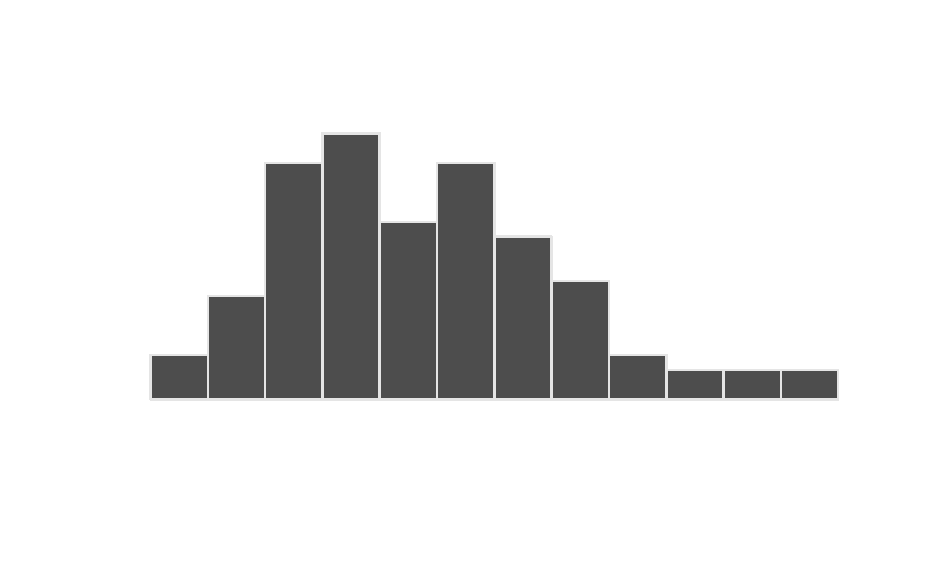
\includegraphics[width=2in]{graphs/bs_bighist}

% {\gr data sample}

% $\swarrow~~~\downarrow~~~\searrow$

% 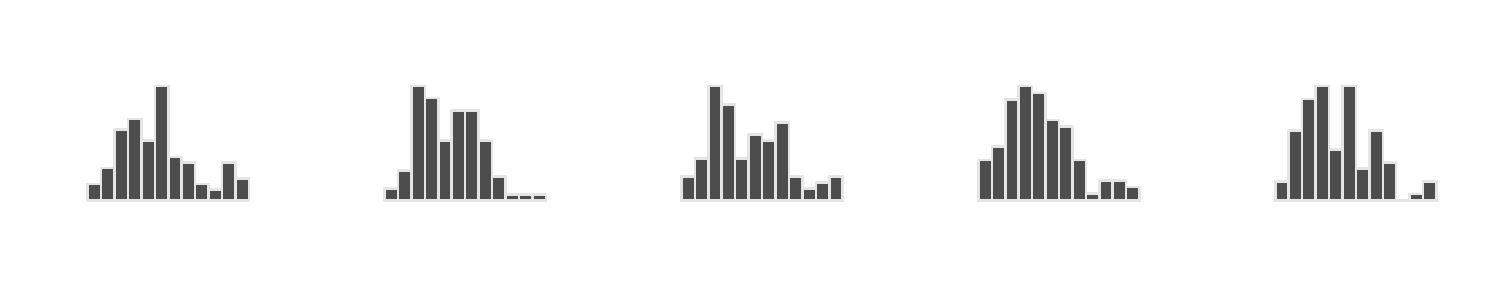
\includegraphics[width=4.25in]{graphs/bs_boothist}

% \gr bootstrap samples
% \end{center}

% You are pretending that the {\it empirical data distribution} is
% the population, and using it to draw alternative samples.
% \end{frame}



% \begin{frame}

% {\bf The {\nv Bayesian} Bootstrap}

% \begin{center}
% 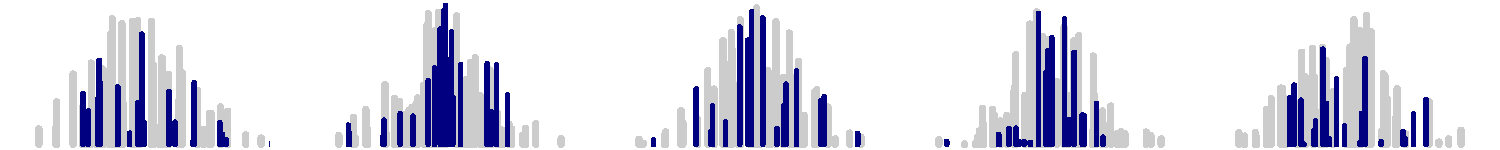
\includegraphics[width=\textwidth]{graphs/bayesbootprior}

% {\gr prior samples}

% $\downarrow~~~~\downarrow~~~~\downarrow$

% 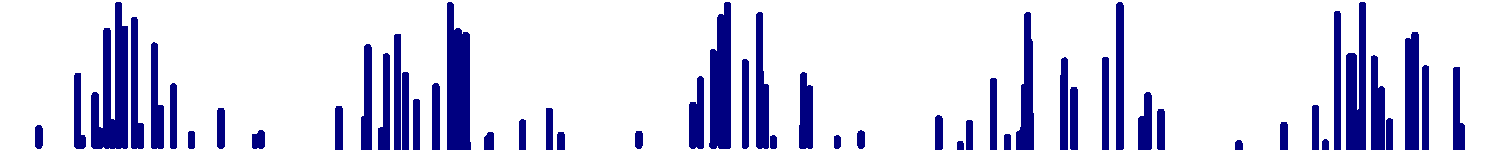
\includegraphics[width=\textwidth]{graphs/bayesbootpost}

% \gr posterior samples
% \end{center}

% You have a nonparametric model over {\it all} possible observations, but then
% use a convenient prior that limits you to observed support.

% \vskip .5cm
% It'll work whenever the standard Bootstrap works: only if the empirical data distribution 
% is a decent substitute for the population.

% \end{frame}

% z <- x <- c()
% dz <- dx <- c()
% for(i in 1:5){
%  x <- cbind(x,rnorm(20))
%  z <- cbind(z,rnorm(50))
%  dx <- cbind(dx,dnorm(x[,i])*runif(20))
%  dz <- cbind(dz,dnorm(z[,i])*runif(50))}

% pdf("graphs/bayesbootprior.pdf",width=10,height=1)
% par(mai=c(0,.2,0,.2),mfrow=c(1,5))
% for(i in 1:5){
%  plot(z[,i],dz[,i],type="h",col="grey80",ylim=c(0,max(c(dx,dz))),
%   xaxt="n",yaxt="n", bty="n",lwd=4,xlab="",ylab="")
%  lines(x[,i],dx[,i],type="h",col="navy",lwd=3)}
% dev.off()

% z <- x <- c()
% dz <- dx <- c()
% for(i in 1:5){
%  x <- cbind(x,rnorm(20))
%  z <- cbind(z,rnorm(50))
%  dx <- cbind(dx,dnorm(x[,i])*runif(20))
%  dz <- cbind(dz,dnorm(z[,i])*runif(50))}

% pdf("graphs/bayesbootpost.pdf",width=10,height=1)
% par(mai=c(0,.2,0,.2),mfrow=c(1,5))
% for(i in 1:5)
%     plot(x[,i],dx[,i],type="h",col="navy",
%      xaxt="n",yaxt="n", bty="n",lwd=4,xlab="",ylab="")
% dev.off()

\begin{frame}

{\bf {\gr Example: } Ordinary Least Squares}

\vskip .5cm
{\it Population} OLS is a posterior functional
\begin{equation*}
\bs{\beta} = (\bm{X}'\bs{\Theta}\bm{X})^{-1}  \bm{X}'\bs{\Theta}\bm{y}
\end{equation*}
where $\bs{\Theta} = \mr{diag}(\bs{\theta})$.  
{\theme This is a random variable. \gr (sample via BB)}

\vskip .75cm
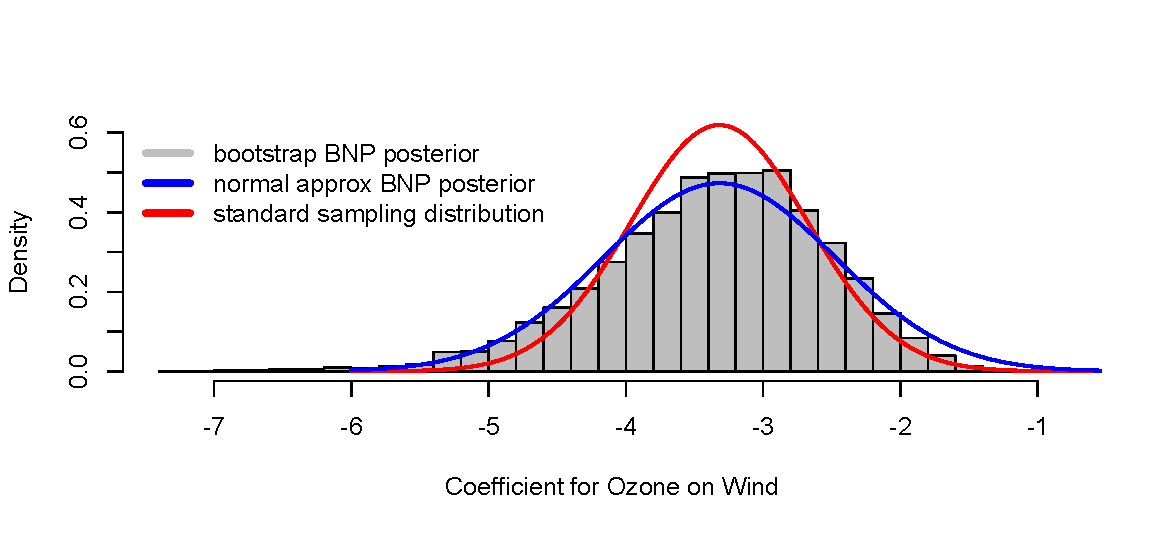
\includegraphics[width=\textwidth]{graphs/ozone}
\end{frame}

% \begin{frame}[fragile]

% {\footnotesize\gr
% \begin{verbatim}
% data(airquality); n <- nrow(airquality)
% B <- 1000; beta <- vector(length=B)
% for(b in 1:B){
%   fit <- lm(Ozone ~., data=airquality, weights=rexp(n))
%   beta[b] <- coef(fit)["Wind"] }
% sampfit <- lm(Ozone ~ ., data=airquality)
% coef <- summary(sampfit)$coef["Wind",1:2]
% x <- as.matrix(cbind(1,na.omit(airquality)[,-1]))
% xxi <- solve(crossprod(x))
% sandwich <- xxi%*%t(x)%*%diag(sampfit$resid^2)%*%x%*%xxi
% hist(beta, col=8, main="", 
%   xlab="Coefficient for Ozone on Wind", 
%   freq=FALSE,ylim=c(0,0.6),breaks=25)
% grid <- seq(-6,5,length=500)
% lines(grid, dnorm(grid,coef[1],coef[2]),col=2,lwd=2)
% lines(grid, dnorm(grid,coef[1],sqrt(sandwich[3,3])),col=4,lwd=2)
% legend("topleft",col=c(8,2),lwd=4, 
%   legend=c("bootstrap BNP posterior",
%            "normal approx BNP posterior",
%            "standard sampling distribution"),bty="n")
% \end{verbatim}
% }

% \end{frame}




\begin{frame}

{\nv \bf What is the blue line? } 

\vskip .5cm
BB sampling is great, but analytic approximations are also useful.

\vskip .25cm
Consider a first-order Taylor series approximation,
\[
\bs{\tilde \beta} = \bs{\hat\beta}+ 
\nabla \bs{\beta}\big |_{\bs{\theta}=\bm{1}} (\bs{\theta} - \bm{1})
\]
where $ \bs{\hat\beta} = [\bm{X}'\bm{X}]^{-1}\bm{X}'y = \bs{\beta}\big|_{ \bs{\theta}=\bm{1}}$ is the sample OLS line.

\vskip .5cm
We can derive {\it exact} posterior moments for $\bs{\tilde \beta}$. e.g.,
\[
\mr{var}(\bs{\beta}) \approx \mr{var}(\bs{\tilde \beta}) = (\bm{X}^{\prime}\bm{X})^{-1}\bm{X}^{\prime}\mr{diag}(\bm{e}^2)\bm{X}^{\prime}(\bm{X}^{\prime}\bm{X})^{-1}
\]
 where $\bm{e}  = \bm{y} - \bm{X}\bs{\hat\beta}$ are the sample OLS residuals.

\vskip .25cm
This is the economist's Huber-White `Sandwich' variance formula.

\vskip .1cm{\gr \hfill
 \small(Lancaster 2003 or Poirier 2011.)}

\end{frame}

\begin{frame}

{\bf{\gr Example:} Heterogeneous Treatment Effects}

\vskip .5cm
{\nv eBay runs lots of experiments:} they make changes to the marketplace (website) for random samples of users.

\vskip .5cm
Every experiment has response $y$ and treatment $d$ {\gr [0/1]}.

\vskip .05cm
In our illustrative example,
$d_i = 1$ for bigger pictures in my eBay.


\vskip .25cm
{\small $i\in{\sf control}: d_i=0$ \hspace{2.5cm} $i\in{\sf treatment}: d_i=1$}

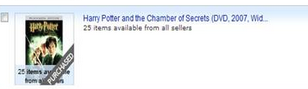
\includegraphics[scale=.5]{graphs/pottersmall}

\includegraphics[scale=.5]{graphs/potterbig}


\vskip .5cm
This is a typical `A/B experiment'.
\end{frame}

\begin{frame}

What is `heterogeneity in treatment effects'? {\gr(HTE)}

\vskip .2cm Different units {\gr [people, devices]} respond differently to some treatment you apply {\gr [change to website, marketing, policy]}.  

\vskip .2cm {\theme I imagine it exists.  }

\vskip .5cm
We know $\bm{x}_i$ about user $i$. {\gr About 400 features in our example.}

\vskip .1cm
\begin{itemize}
\item Their previous spend, items bought, items sold...
\item Page view counts, items watched, searches, ...
\item All of the above, broken out by product, fixed v. auction, ...
\end{itemize}

\vskip .1cm Can we accurately measure heterogeneity: index it on $\bm{x}$?

\end{frame}



\begin{frame}

{\bf Treatment effect regression}

\vskip .5cm
{\theme Potential outcomes: } $\upsilon_{i}(d)$ is the response for user
$i$ if $d_i = d$.

\vskip .25cm
We'd love to model $\ds{E}[\upsilon_{i}(1)- \upsilon_{i}(0) | \bm{x}_i]$, but we can't directly.  

\vskip .5cm
Since $d \indep [\bm{x},\bs{\upsilon}]$, a good alternative is to consider 
\[
\ds{E}[\upsilon_{i}(1)|d_i=1,\bm{x}_i] - \ds{E}[\upsilon_{i}(0) |d_i=0,\bm{x}_i].
\]
Even simpler, just diff the OLS projections for each group
\[
\bs{\beta}_{\sf t} - \bs{\beta}_{\sf c} = (\bm{X}_{\sf t}'\bs{\Theta}_{\sf t}\bm{X}_{\sf t})^{-1}  \bm{X}_{\sf t}'\bs{\Theta}_{\sf t}\bm{y}_{\sf t} -
 (\bm{X}_{\sf c}'\bs{\Theta}_{\sf c}\bm{X}_{\sf c})^{-1}  \bm{X}_{\sf c}'\bs{\Theta}_{\sf c}\bm{y}_{\sf c}
\]

%{\gr \small See Taddy, Gardner, Chen, Draper 2014 for alternative linear projections.}

\end{frame}

\begin{frame}

% Since $\bs{\beta}_{\sf t} \indep \bs{\beta}_{\sf c}$, our results on BNP analysis of OLS apply directly.  Or you can bootstrap, but it takes a long time.

% \vskip .25cm
e.g., coefficient on {\it [made purchase this year]} vs an intercept:

\vskip .5cm
{\footnotesize\it
\gr million users:~~~~~~~~~~~~~~7.45~~~~~~~~~~~~~~~~~~~~~~~10.97~~~~~~~~~~~~~~~~~~~~~13.22}
\begin{center}
\vskip -.25cm
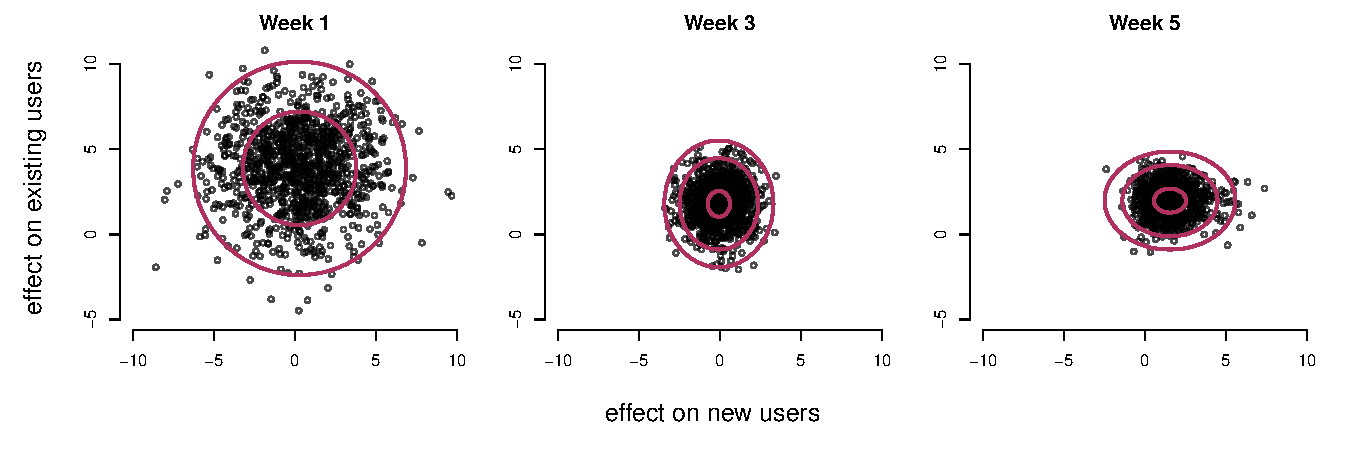
\includegraphics[width=.9\textwidth]{graphs/gammapost}
\end{center}

{\gr Sample is from posterior, contours are normal approximation.}


\end{frame}

\begin{frame}

%$\bs{\beta}_{\sf t} - \bs{\beta}_{\sf c}$ is a statistic we care about, even if the truth is nonlinear.

%\vskip .25cm 
The most basic application of an A/B experiment is estimating the average treatment effect,
\[
\text{ATE} = \ds{E}[\upsilon({\sf t})] -
\ds{E}[\upsilon({\sf c})] 
\] 
The usual estimator is $\bar{y}_{\sf t} - \bar{y}_{\sf c}$.
But many authors  advocate instead the `regression adjusted' $\bm{\bar x}'(\bs{\hat\beta}_{\sf t} - \bs{\hat\beta}_{\sf c})$  {\gr \small (Lin, Berk\texttt{+}, Deng\texttt{+}, 2013)}.

\vskip .25cm
Both are [frequentist] unbiased. 

\vskip .5cm
 But quantifying uncertainty about the regression adjustment, and any variance reduction it provides, is tough without assumptions.  

\end{frame}

\begin{frame}

From our BNP persepective, both the usual and adjusted ATE estimators are random functions of the DGP.
\begin{eqnarray*}
\text{ATE}^\text{obs}_g &=& 
\frac{1}{|\bs{\theta}_{\sf t}|}\bs{\theta}_{\sf t}'\bm{y}_{\sf t} - \frac{1}{|\bs{\theta}_{\sf c}|}\bs{\theta}_{\sf c}'\bm{y}_{\sf c}
\\
\text{ATE}^\text{lin}_g &=& \frac{1}{|\bs{\theta}|}\bs{\theta}'\bm{X}\bigg( (\bm{X}_{\sf t}'\bs{\Theta}_{\sf t}\bm{X}_{\sf t})^{-1}  \bm{X}_{\sf t}'\bs{\Theta}_{\sf t}\bm{y}_{\sf t} - (\bm{X}_{\sf c}'\bs{\Theta}_{\sf c}\bm{X}_{\sf c})^{-1}  \bm{X}_{\sf c}'\bs{\Theta}_{\sf c}\bm{y}_{\sf c}\bigg).
\end{eqnarray*}

Using our usual tricks, we can resolve any \textit{controversy}:
\[
\mr{var}\left(\text{ATE}^\text{lin}_g\right) \approx \mr{var}(\text{ATE}^\text{obs}_g) - \left( \frac{R^2_{\sf t}s^2_{\bm{y}_{\sf t}}}{n^2_{\sf t}} +  
\frac{R^2_{\sf c}s^2_{\bm{y}_{\sf c}}}{n^2_{\sf c}} \right),
\]
so that big variance reduction comes only for small sample $n_{\sf d}$ or large $R_{\sf d}^2 = \mr{cor}(y_{\sf d},\hat y_{\sf d})$.  {\theme In digital experiments we have big samples and low signal, so we shouldn't expect much variance reduction.}

\end{frame}

\begin{frame}


{\bf {\gr Example:} Decision Trees}

\vskip .5cm
Trees are great: nonlinearity, deep interactions, heteroskedasticity.

\begin{center}
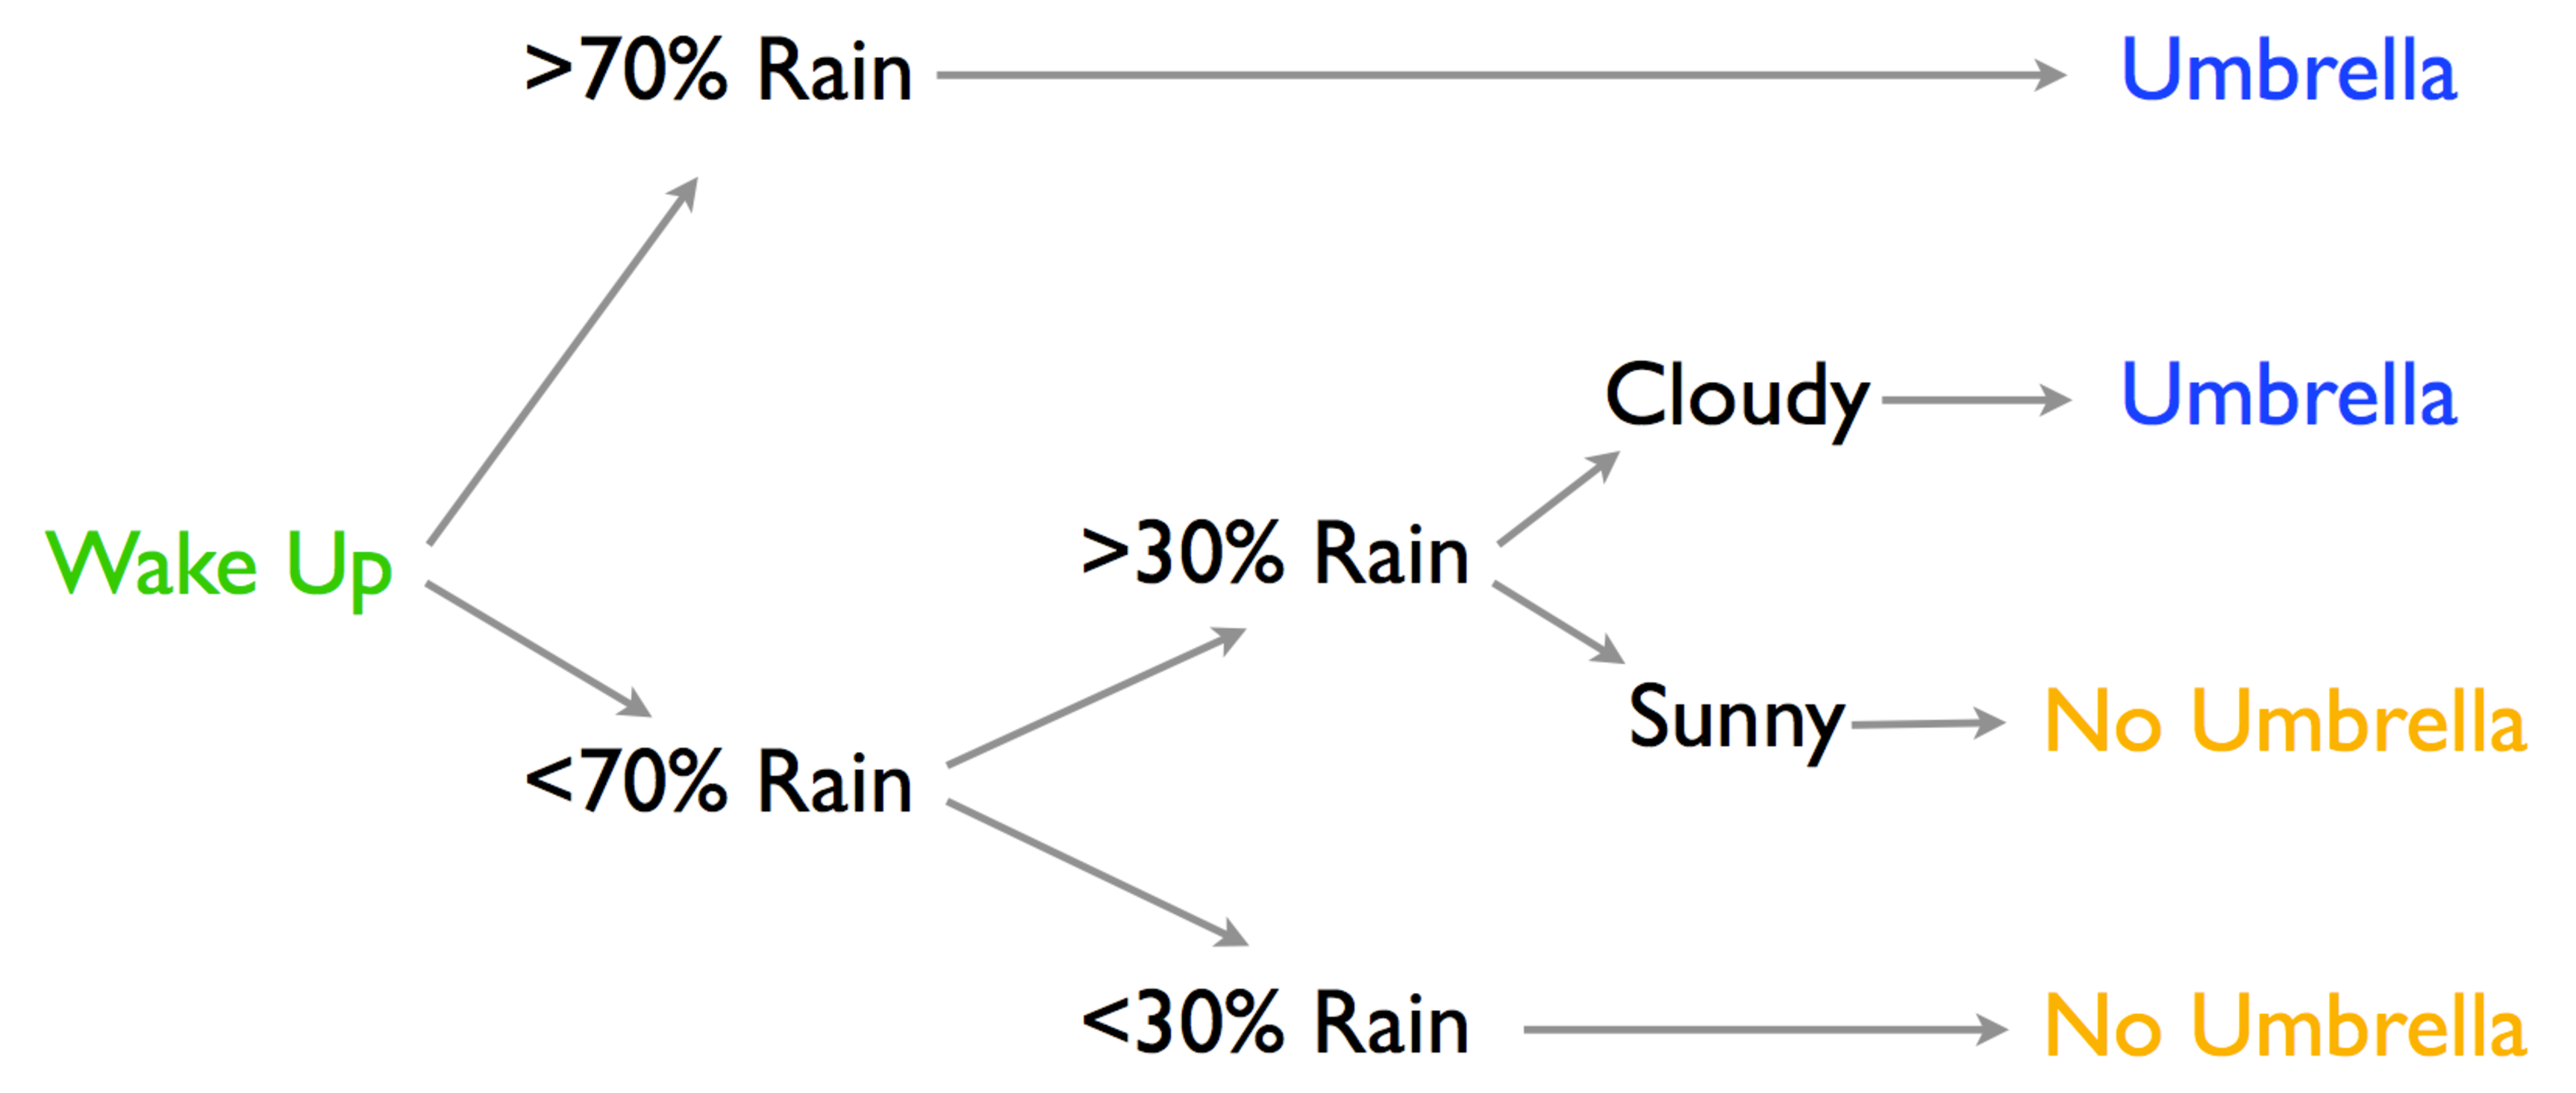
\includegraphics[width=4in]{graphs/umbrella}
\end{center}

The `optimal' decision tree is a statistic we care about {\gr (s.w.c.a)}.


\end{frame}


\begin{frame}


{\bf {\theme CART:} greedy growing with optimal splits}

\vskip .5cm
Given node $\{\bm{x}_i,y_i\}_{i=1}^n$ and DGP weights $\bs{\theta}$,
find $x$ to minimize 
\begin{align*}
|\bs{\theta}|\sigma^2(x, \bs{\theta} ) &= \sum_{k \in \mathrm{left}(x)} \theta_k (y_k - \mu_{\mathrm{left}(x)})^2 \\&+ \sum_{k \in \mathrm{right}(x)} \theta_k (y_k - \mu_{\mathrm{right}(x)})^2
\end{align*}
for a regression tree.  Classification impurity can be Gini, etc.


\vskip .5cm
Population-CART might be a statistic we care about.


\vskip .1cm{\gr 
Or, in settings where greedy CART would do poorly (big $p$), \\a randomized splitting algorithm might be a better s.w.c.a.}



\end{frame}


\begin{frame}[fragile]

{\bf \theme Bayesian Forests: \bk a posterior for CART trees}

\vskip .25cm
For $b=1 \dots B$: \\
   ~~~~~~~~~~$\bullet$ draw $\boldsymbol{\theta}^b \stackrel{iid}{\sim} \mathrm{Exp}(\mathbf{1})$
   \\
   ~~~~~~~~~~$\bullet$ run weighted-sample CART to get $\mathcal{T}_b = \mathcal{T}(\boldsymbol{\theta}^b)$
 
\vskip .5cm\small 
~~~~~~~~~~~~~~~~~~~~~{\it one tree~~~~~~~~~~~~~~~~~~~~~~~~~~~~~~~~~~posterior mean}\\

\includegraphics[height=1.75in]{graphs/MCtreedraw}   
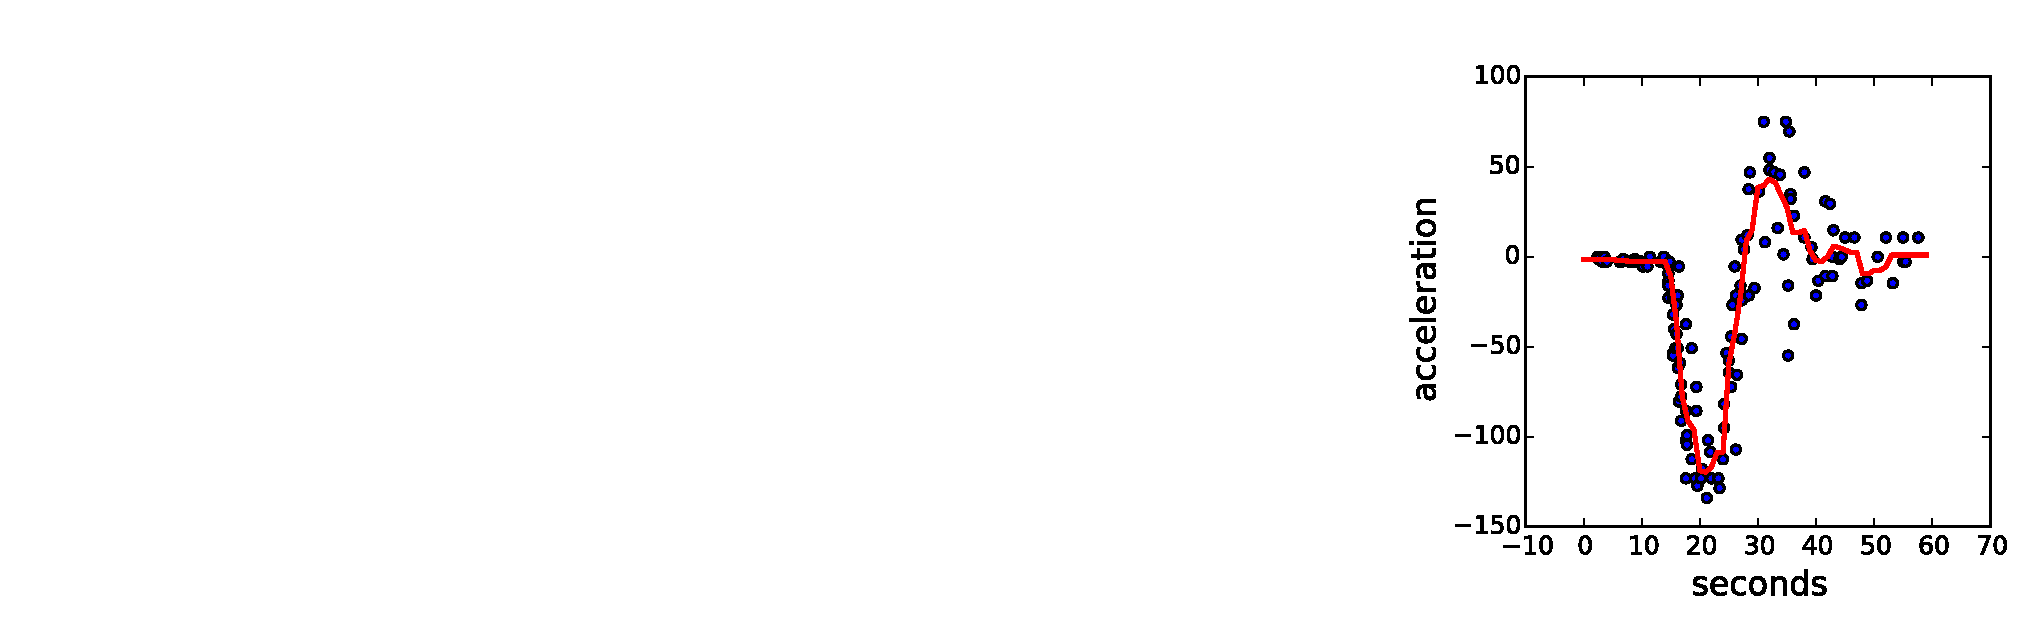
\includegraphics[height=1.75in]{graphs/MCbforest}   

\vskip .25cm{
Random Forest $\approx$ Bayesian forest $\approx$ posterior over CART fits.}

\vskip -.5cm

\end{frame}



\begin{frame}

{\bf Theoretical {\theme trunk} stability}

\vskip .5cm

Given forests as a posterior, 
we can start talking about {\it variance}.

\vskip .1cm

Consider the first-order approximation
\begin{eqnarray*}
\sigma^2(x,\bs{\theta}) \approx& \sigma^2(x,\boldsymbol{1}) + \nabla \sigma^2\big |_{\boldsymbol{\theta}=\mathbf{1}} (\boldsymbol{\theta} - \boldsymbol{1}) \\ &=  \frac{1}{n}\sum_i \theta_i \left[y_i - \bar{y}_i(x)\right]^2
\end{eqnarray*}
with $\bar y_i (x)$ the sample mean in $i$'s node when splitting on $x$.

\vskip .1cm
Based on this approx, we can say that for data at a given node, 
\begin{equation*}\theme
\mathrm{p}\left(\text{optimal split matches sample CART}\right) \gtrsim 1 - \frac{p}{\sqrt{n}} e^{-n},
\end{equation*}
with $p$ split locations and $n$ observations.  

\vskip .2cm
{\gr\small (Taddy,  Chen, Yu, Wyle 2015)}

\end{frame}

\begin{frame}

{\bf California Housing Data}


\vskip .5cm

20k observations on median home prices in zip codes.

\vskip .5cm

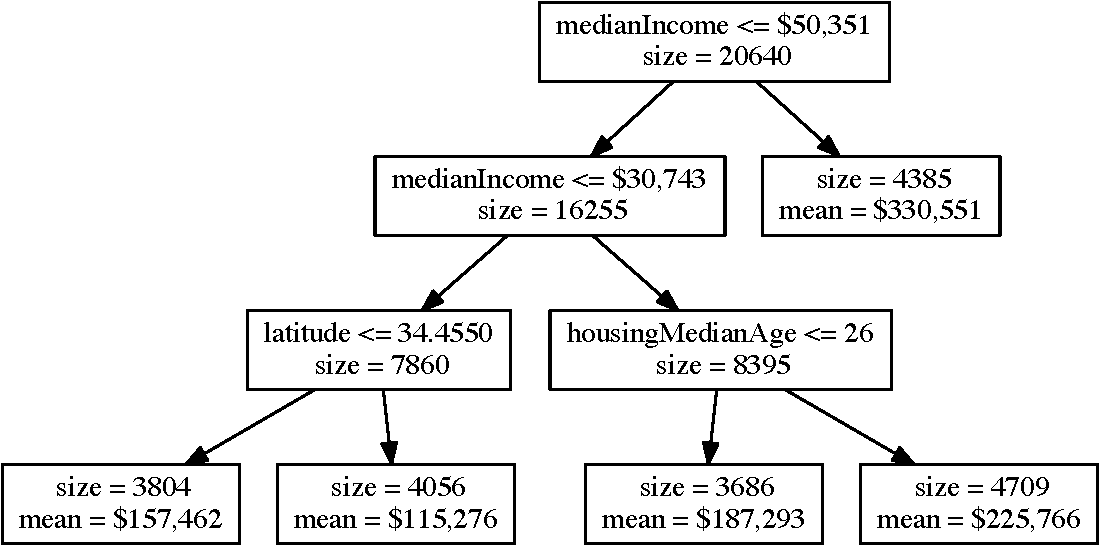
\includegraphics[width=\textwidth]{graphs/ca_trunk}

\vskip .5cm
\hfill Above is the trunk you get setting min-leaf-size of 3500.

\end{frame}

\begin{frame}

\begin{columns}

\begin{column}{2.15in}
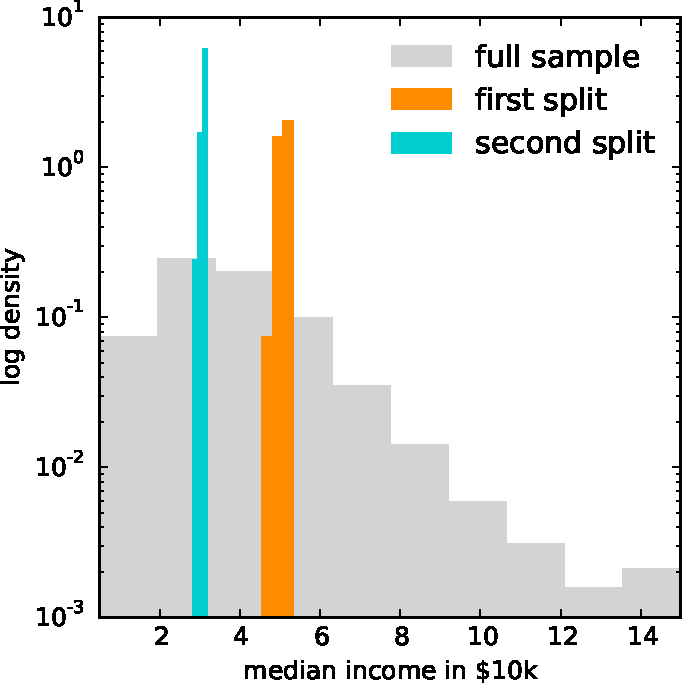
\includegraphics[width=2.5in]{graphs/ca_splits}
\end{column}

\begin{column}{2in}
\begin{itemize}
\item sample tree occurs 62\% \\of the time.  
\vskip .5cm
\item 90\% of  trees split on income twice, \\and then latitude. 

\vskip .5cm
\item 100\% of trees have 1st 2 splits on median income.  
\end{itemize}
\end{column}

\end{columns}


\vskip 1cm
~~~~Empirically and theoretically: trees are stable, at the trunk.
\vskip -1cm

\end{frame}

\begin{frame}

{\bf Random Forest {\theme bottlenecks}}

\vskip .5cm
RFs (or BFs) are awesome, but when the data are too big to fit in memory or on a single machine they get extremely expensive.\\ {\gr \small (e.g., Google PLANET, Panda 2009)}.

\vskip .5cm
A common solution is a `sub-sampling forest': instead of drawing with-replacement, or re-weighting, draw $m \ll n$ sub-samples.

\vskip .5cm
This defeats the whole purpose of trees: these are rules that are designed to grow in complexity with the amount of data available. {\gr(that's why we bother storing so much data!)}

\vskip .5cm If you starve the individual trees of data you lose.

\end{frame}

% \begin{frame}
% \begin{adjustwidth}{-.5in}{}
% \vskip -.6in
% 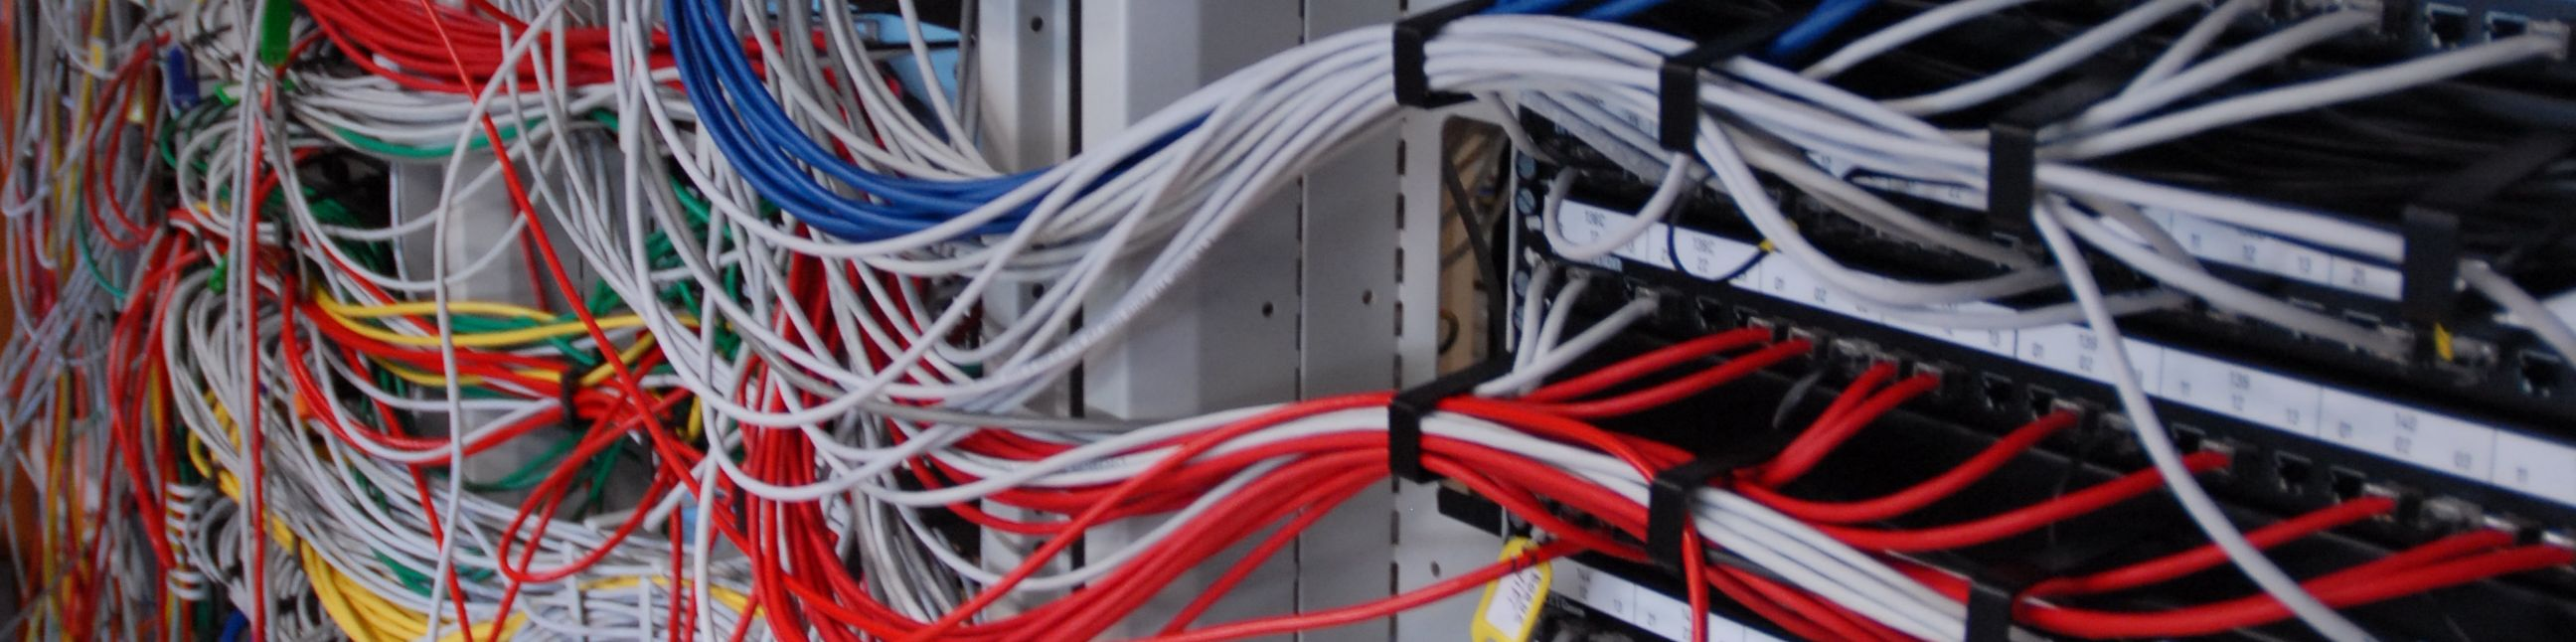
\includegraphics[width=6in]{graphs/broadband}
% \end{adjustwidth}

% \vskip .6cm

% { \bf Data Distribution and Big Data}

% \vskip .5cm
% {\nv Distributed}: independent computations on many datasets.\\

% \vskip .1cm
% For truly {\nv Big Data} we need distributed algorithms.

% \vskip .5cm
% The trick is to find strategies for distribution so that local-machine calculations are as relevant as possible to the global inference question:
% only data that needs to be together is together.

% \end{frame}



\begin{frame}

{\bf Empirical Bayesian Forests ({\theme EBF})}

\vskip .5cm
RFs are expensive.  Sub-sampling hurts bad.

\vskip .25cm
{Instead:}
\begin{itemize}
\item fit a single tree to a shallow {\nv trunk}.  
\item Map data to each {\nv branch}.  
\item Fit a full  forest on the smaller branch datasets.
\end{itemize}

\vskip .25cm
Since the trunks are all similar for each tree in a full forest,
our EBF looks nearly the same at a fraction of computational cost.

\vskip .5cm
It's an updated version of classical {\theme Empirical Bayes}: \\ ~~~use plug-in estimates at high levels in a hierarchical model, \\~~~focus effort at full Bayesian learning for the the hard bits.


\end{frame}

\begin{frame}

{\bf OOS predictive performance on California Housing}




\begin{center}
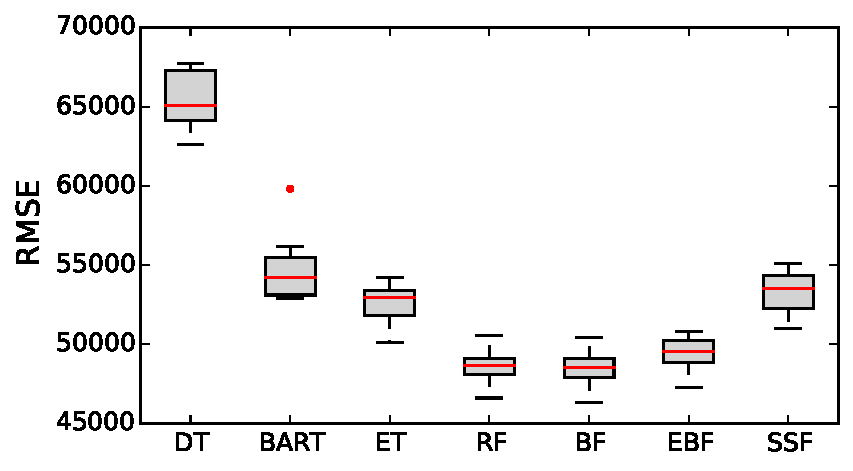
\includegraphics[width=.85\textwidth]{graphs/ca_rmse}
\end{center}

Here EBF and BF give nearly the same results.  {\it SSF does not.}

\vskip .25cm
EBFs crunch more data faster without hurting performance.


\end{frame}


\begin{frame}

{\bf EBFs work all over the place}

\vskip .5cm
\begin{minipage}{0.5\linewidth}
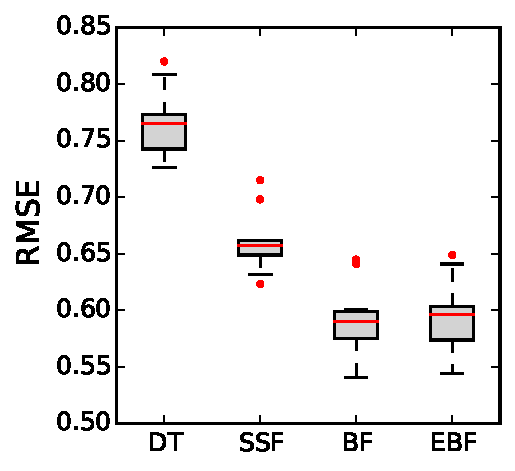
\includegraphics[width=\textwidth]{graphs/wine}
\end{minipage}
~~
\begin{minipage}{0.4\linewidth}
{\footnotesize
\begin{tabular}{c c | l}
$\overline{\text{RMSE}}$  & \% WTB & \\
\cline{1-2}\rule{0pt}{3ex} 
0.5905 &  0.0 & BF \\
0.5953 &  0.8 & EBF \\
0.6607 & 11.9 & SSF \\
0.7648 & 29.5 & DT \\
\end{tabular}}
\end{minipage}

\vskip .5cm
\hfill Predicting wine rating from chemical profile

\end{frame}


\begin{frame}

{\bf EBFs work all over the place}

\vskip .5cm
\begin{minipage}{0.5\linewidth}
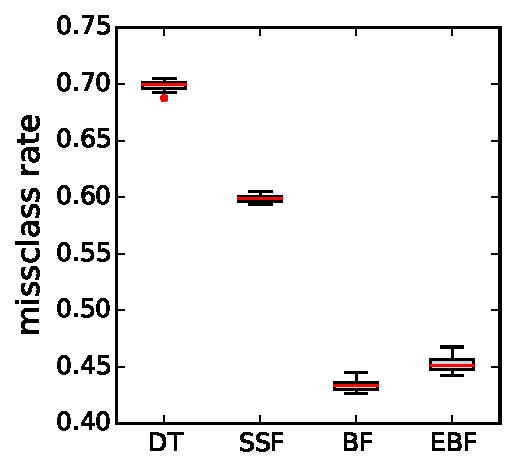
\includegraphics[width=\textwidth]{graphs/beer}
\end{minipage}
~~
\begin{minipage}{0.4\linewidth}
{\footnotesize
\begin{tabular}{c c | l}
$\overline{\text{MCR}}$  & \% WTB & \\
\cline{1-2}\rule{0pt}{3ex} 
0.4341 &  0.0 & BF \\
0.4531 &  4.4 & EBF \\
0.5989 & 38.0 & SSF \\
0.6979 & 60.8 & DT \\
\end{tabular}}
\end{minipage}

\vskip .5cm
\hfill or beer choice from demographics

\end{frame}

\begin{frame}

{\bf Choosing the trunk depth}


\vskip .5cm
Distributed computing perspective: {\theme fix only as deep as you must!}

\vskip .1cm
How big is each machine? Make that your branch size.

\vskip .75cm
{\small
\begin{tabular}{c | c c c | c c c | c c c}
& \multicolumn{3}{l|}{CA housing} & \multicolumn{3}{l|}{Wine} &\multicolumn{3}{l}{Beer} \\
\cline{2-10} \rule{0pt}{3ex} 
\!\!\!\!\!\!{\it Min Leaf Size in $10^3$} & 6 & 3 & 1.5 & 2  & 1 & 0.5 & 20 & 10 & 5\\
\!\!\!\!\!\!{\it \% Worse Than Best} & \!1.6 & \!2.4 & \!4.3 & \!0.3 & \!0.8 & \!2.2 & \!1.0 & \!4.4 & \!7.6 
\end{tabular}}

\vskip .5cm
Still, open questions:  e.g., more trees vs shallower trunk?

\end{frame}

\begin{frame}

{\bf Catching {\theme Bad Buyer Experiences } at eBay}

\vskip .5cm
BBE: `not as described', delays, etc.

\vskip .1cm
$\mathrm{p}(\text{BBE})$
is a key input to search rankings, and elsewhere.

\vskip .5cm
Big Data axiom:  best way to improve prediction is more data.  

\vskip .1cm 
{\gr (a.k.a. `data beats model' )}


\vskip .5cm
On 200 million transactions,  EBF with 32 branches yields a\\ 1.5\% drop in misclassification over the SSF alternatives.  

\vskip .5cm
EBFs via Spark $\Rightarrow$ more data in less time.
\vskip .1cm 
Putting it into production requires some careful engineering, \\but this really is a very simple algorithm.  {\theme Big gain, little pain.} 

\end{frame}


\begin{frame}

{ \bf {\theme Back to HTE:}  Treatment Effect Trees}


\vskip .5cm
Recall our earlier example: A/B experiment with user covariates $\bm{x}_i$.

\vskip .35cm
Athey\texttt{+}Imbens propose indexing user HTE by fitting CART to
\[
y^\star_i = y_i \frac{d_i - q}{q(1-q)} = \left\{
\begin{array}{cc}
y_i/(1-q) &\text{if~} d_i=0\\
y_i/q &\text{if~} d_i=1
\end{array}\right.
\]
where $q$ is the probability of treatment ($2/3$ in our example).

\vskip .35cm
This works because
\[
\ds{E}[y^\star_i | \bs{\upsilon}_i] = 
%q \upsilon_i(1)\frac{1 - q}{q(1-q)} - (1-q) \upsilon_i(0)\frac{q}{q(1-q)}
\upsilon_i(1)- \upsilon_i(0).
\]
% {\gr Recall: $\upsilon_i(d)$ is the potential outcome for user $i$ if $d_i = d$.}

How sure are we of the fitted tree?  {\nv Bayes forest is a posterior.}
\end{frame}

% \begin{frame}

% A\texttt{+}I use Cross Validation to prune a single CART tree.

% \vskip .1cm
% But: CV can perform poorly for selection of {\it unstable} models.

% \vskip .1cm
% {\gr 
% Breiman 1996 is the classic paper on this and it's the motivation behind Random Forests in Breiman 2001: averaging beats pruning.}


% \vskip .5cm
% How good are the trees in this case?

% \vskip .1cm
% We can apply the Bayesian bootstrap (i.e., fit a BF) to assess {\it posterior uncertainty} about the selected treatment-effect trees.

% \vskip .5cm
% {\gr\small (BTW if you don't need a single tree, a better solution might be to just partition by predicted treatment effect from the forest, say $>$ or $<$ zero.)}
% \end{frame}

\begin{frame}


e.g., Pruned CART with after one week:
\begin{center}
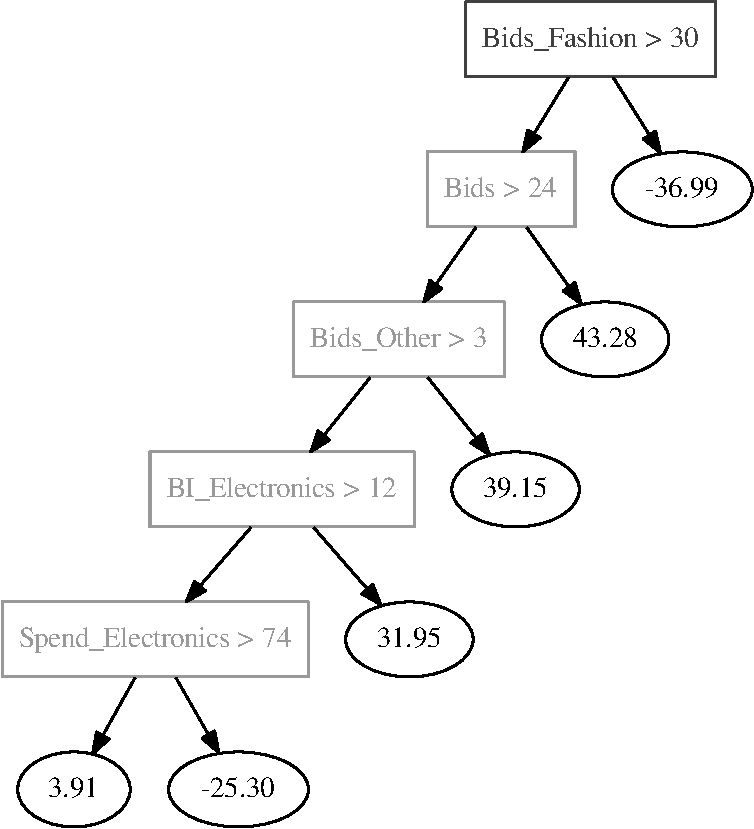
\includegraphics[width=.5\textwidth]{graphs/samptree_week1}
\end{center}
\hfill prob variable is node in tree: {\color{black!50} $\mr{p} <\tfrac{1}{3}$},
{\color{black!75}  $\mr{p} \in
\left[\tfrac{1}{3},\tfrac{1}{2}\right)$}, and {\color{DarkRed}  $\mr{p}
\geq \tfrac{1}{2}$}.
\end{frame}

\begin{frame}

After 5 weeks the tree is much more stable.
\begin{center}
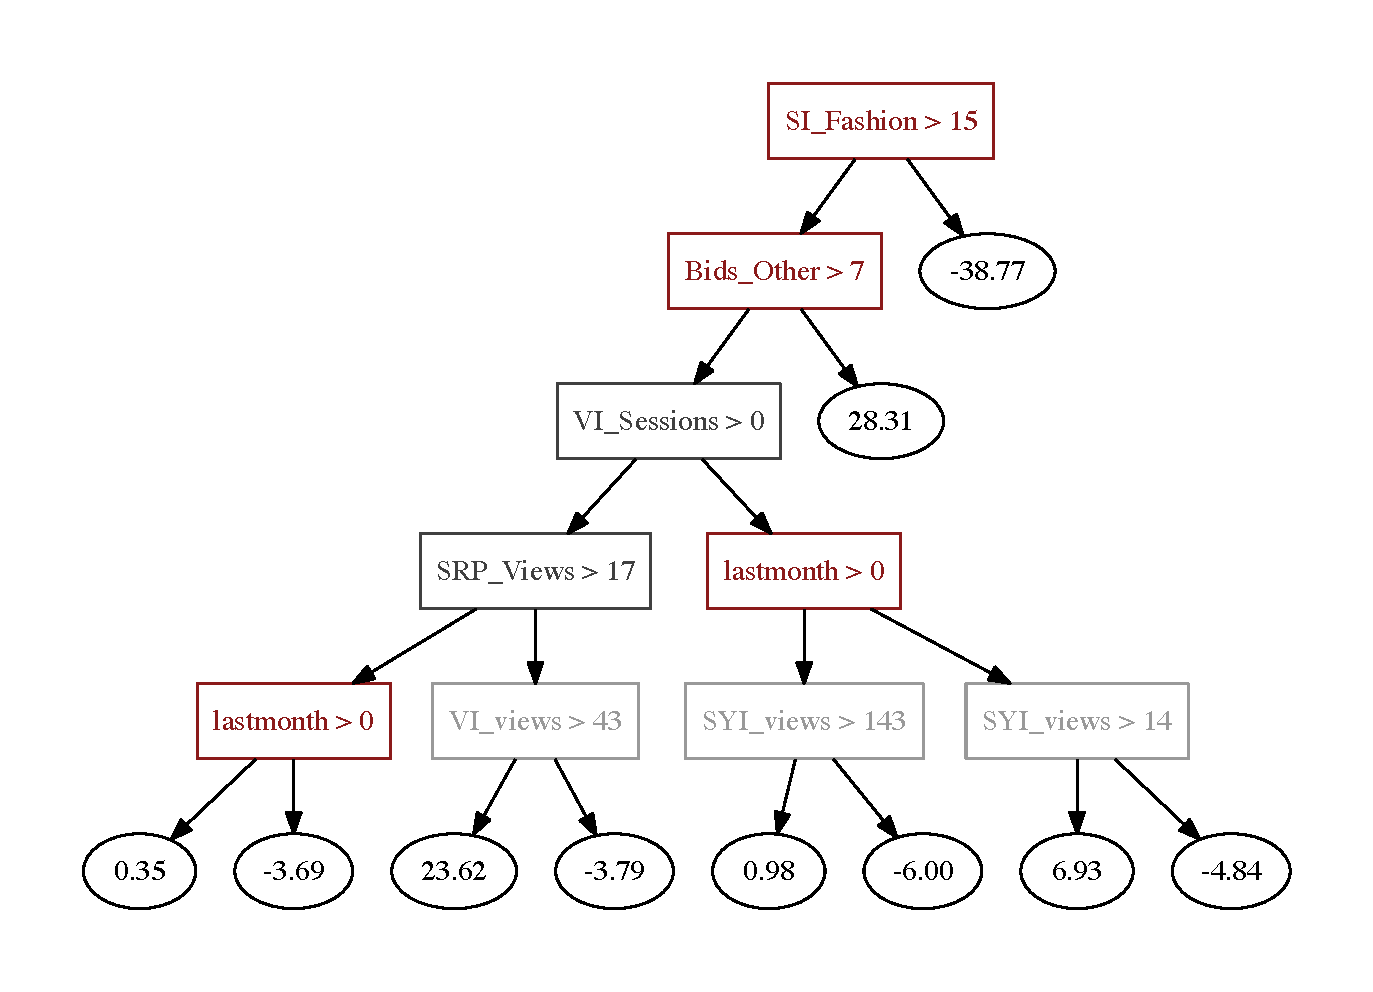
\includegraphics[width=.9\textwidth]{graphs/samptree_week5}
\end{center}

\hfill But you should still use a forest below a certain point.
\end{frame}
 
\begin{frame}

{\it It is wise to look to the full forest instead:}


\vskip .75cm
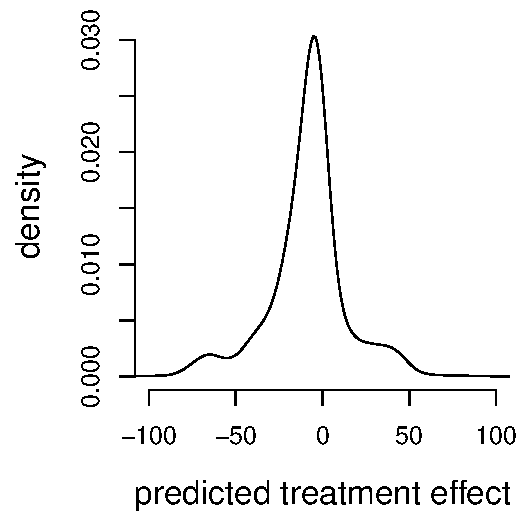
\includegraphics[width=.225\textwidth]{graphs/effdens306894}\!
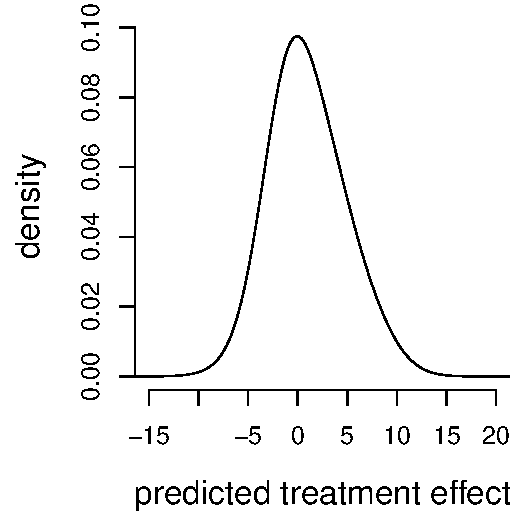
\includegraphics[width=.225\textwidth]{graphs/effdens227148}\!
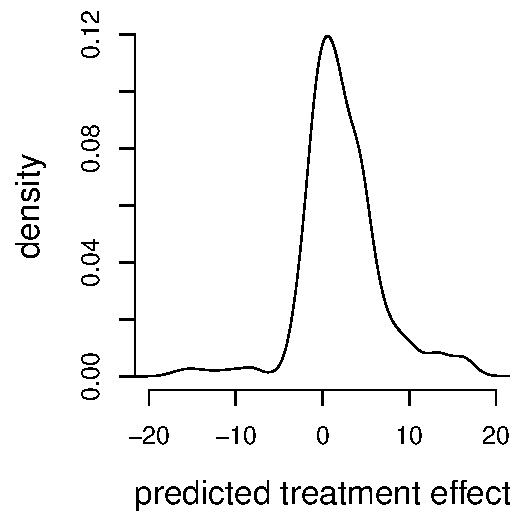
\includegraphics[width=.225\textwidth]{graphs/effdens17689}\!
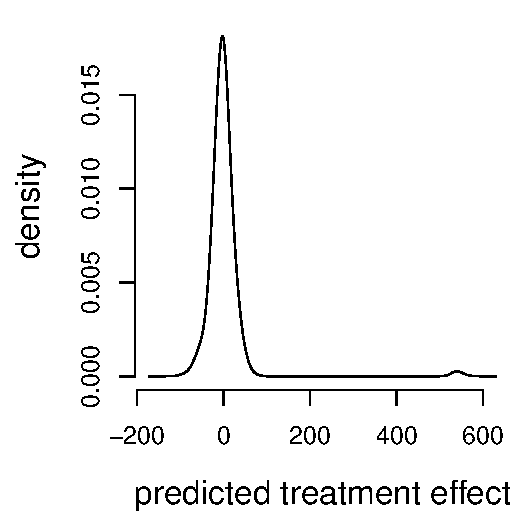
\includegraphics[width=.225\textwidth]{graphs/effdens314303}\!


Treatment effect posteriors for sampled users (5-week data). 

\vskip .5cm

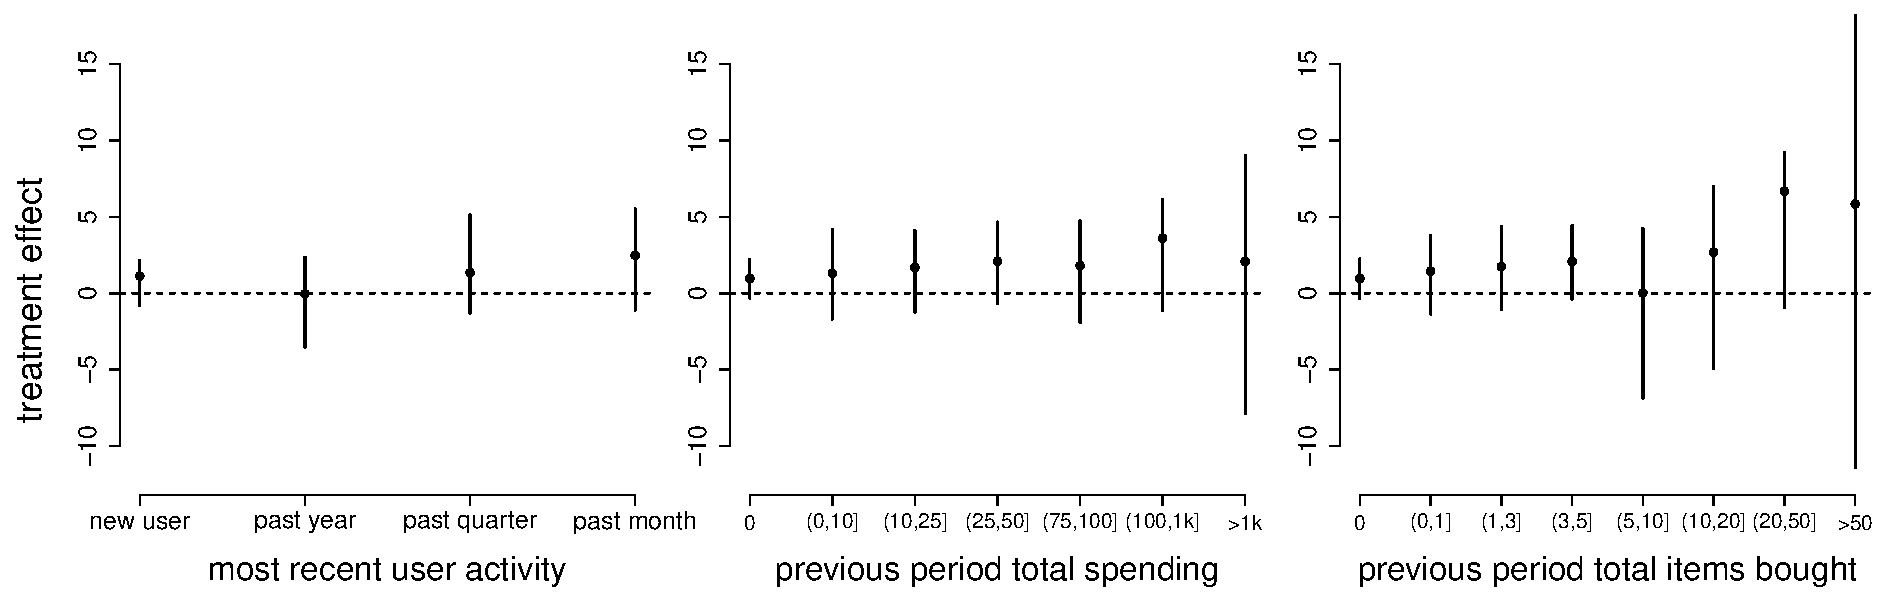
\includegraphics[width=\textwidth]{graphs/maineff}

Variable average effects for three important user features.
\end{frame}

\begin{frame}

{\bf Heavy tails and semiparametric extensions}

\vskip .5cm
In some settings we have really heavy tailed data.

\vskip .25cm
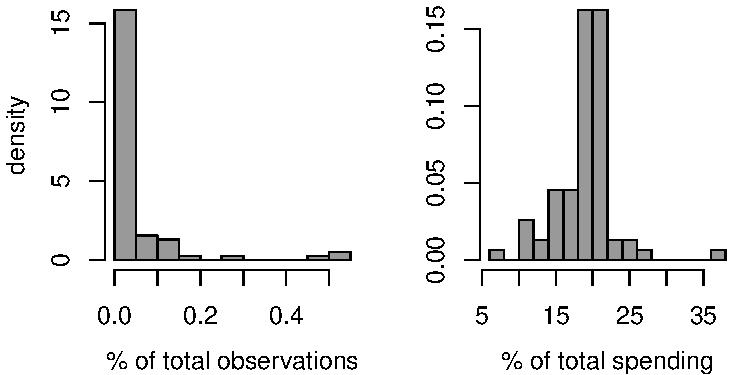
\includegraphics[width=\textwidth]{graphs/gt2k_proportion.pdf}

\vskip .25cm
The standard bootstrap fails for infinite variance distributions.  

\vskip .25cm
We should suspect our Bayesian bootstrap will have similarly bad frequentist properties.  {\gr e.g., the posterior will not be consistent.}
\end{frame}

\begin{frame}

{\bf Semi-parametrics: only model where you really need it.}

\vskip .5cm
We can replace our DGP with a model that includes a parametric tail above some threshold $u$:
\[
\mr{p}(z ) = \frac{1}{|\bs{\theta}|}
\sum_{l=1}^L \theta_l \ds{1}{[z =
\zeta_l]} + \frac{\theta_{L+1}}{|\bs{\theta}|} \theme \mathrm{GPD}(z-u;~\xi,~\sigma)\ds{1}{[z \geq u]}
\]
where $\mathrm{GPD}(\cdot;~\xi,~\sigma)$ is the generalized Pareto density function 
\[
\mathrm{p}(y) = \frac{1}{\sigma}\left( 1 + \xi \frac{y}{\sigma}\right)^{-(\frac{1}{\xi} + 1)}
\]
with $\xi>0$  the tail index and $\sigma>0$  the scale.  

\end{frame}

\begin{frame}
{Inference for tail parameters}

Everything for the weights is as before 
{\gr (exponential posterior)}.

\vskip .25cm
For the GPD tail parameters, we use the prior
\begin{equation*}\label{eq:gpdrefprior}
\pi(\sigma,\xi) = \frac{1}{\sigma}\xi^{a-1}(1-\xi)^{b-1}\mathds{1}_{\xi \in (0,1)},
\end{equation*}

For noninformative inference, use $a=b=1$.  But it is cooler to use a bank of related `background' tail transactions to estimate $\hat\alpha,\hat \beta$.


\vskip .25cm
We have a super simple independence MH posterior sampler \\that is based upon re-sampling from a parametric bootstrap.

\vskip .1cm
Or, you can use a laplace approximation.

\end{frame}

\begin{frame}

Inference for the mean exeedance $\lambda = \sigma/(1-\xi)$, \\beyond $u=\$9000$, in one of our treatment groups.

\begin{center}
{\footnotesize ~~~$a=1,~ b=1$~~~~~~~~~~~~~$a=9,~ b=9$~~~~~~~~~~~$a=80,~ b=80$}
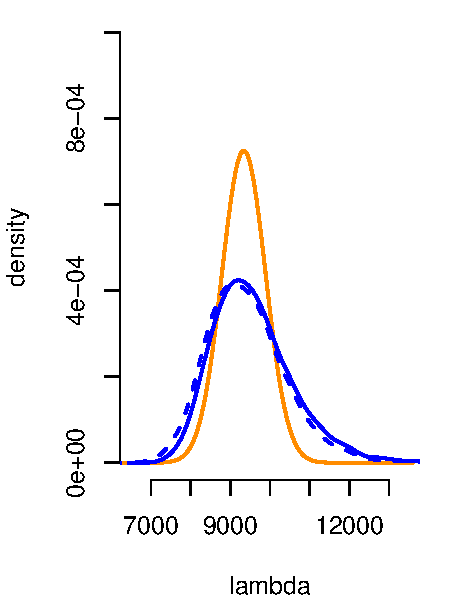
\includegraphics[width=.34\textwidth]{graphs/tail33203-u9000-a1-b1.pdf}\!\!\!\!\!\!\!
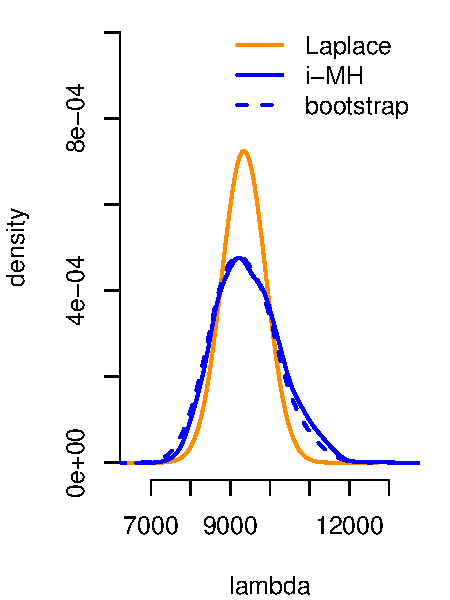
\includegraphics[width=.34\textwidth]{graphs/tail33203-u9000-a9-b9.pdf}\!\!\!\!\!\!\!
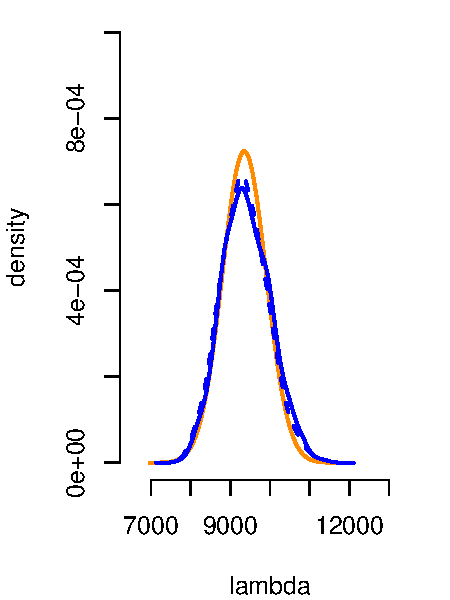
\includegraphics[width=.34\textwidth]{graphs/tail33203-u9000-a80-b80.pdf}
\end{center}

These results can be used for inference about the overall mean, via
{\small $\ds{E}\mu = \tfrac{1}{m+n}\sum_{i=1}^m z_i + \frac{n}{m+n}(u +
\ds{E}\lambda)$ \&
$
\mr{var} \mu = \ds{E}[\mr{var}(\mu|\lambda)] + \mr{var}(\ds{E}[\mu|\lambda]).
$}

\end{frame}

\begin{frame}


Average  performance over 20 resamples
of $N=5000$ from each of 25 treatment group samples, containing
1-3$\times10^5$ observations. 

\begin{center}
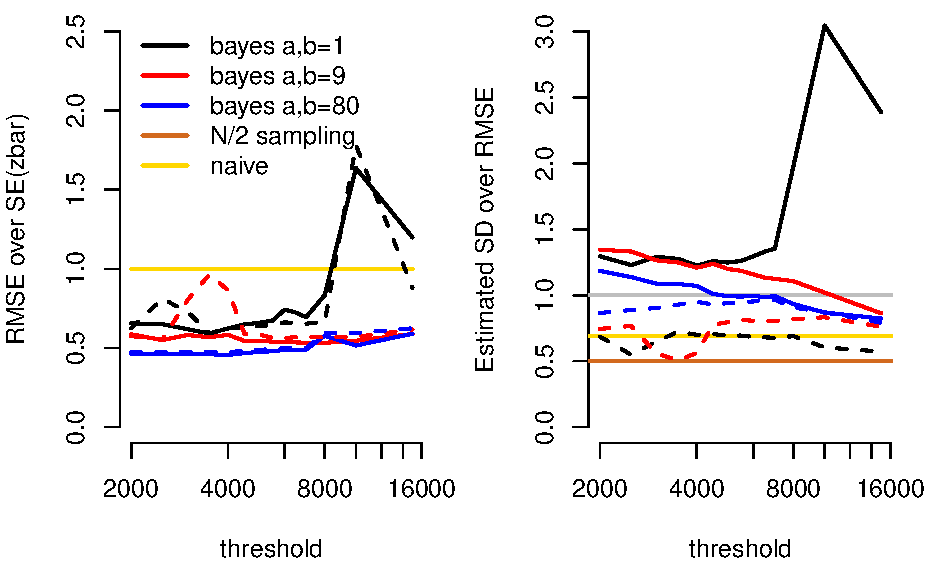
\includegraphics[width=.85\textwidth]{graphs/performance.pdf}
\end{center}

We make gains of up to 50\% in RMSE relative to $\bar z$, and also have better coverage than either $\mr{sd}(z)/\sqrt{n}$ or the $\frac{n}{2}$-of-$n$ bootstrap.
\vskip -.5cm
\end{frame}

\begin{frame}

{\bf Choosing the threshold}

\vskip .5cm
We show consistency for the analogous \textit{frequentist semiparametric bootstrap} (explains our nice coverage) when 
$u_N = O(N^{\xi/(1+2\delta\xi)})$.

\vskip .5cm
In this limit, $\sigma_N = \xi u_N$.  So, one can increase $u$ until this  holds. {\gr Indeed, it  holds roughly in our examples for good performing $u$.}

\vskip  .5cm
But in finite sample practice, it seems wise to try a few $u$ \\and use one in the range where inference is stable.

\end{frame}

\begin{frame}
{Semi-parametrics in treatment effect estimation}


Semiparametric inference makes a big difference in A/B analysis.\\
 Looking at ATEs, $\mu_1 - \mu_2$, in a few example experiments:

\vskip .25cm
\hfill {\footnotesize {\bl sp-bayes}, {\bk capped}, {\rd naive}}
\begin{center}\vskip -.5cm
\!\!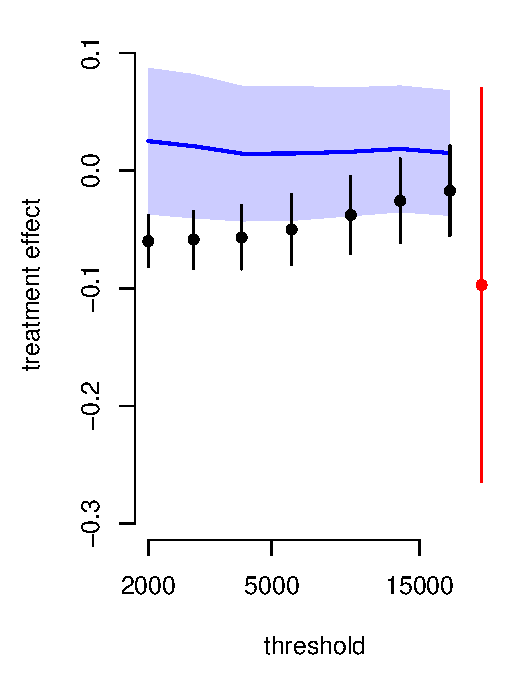
\includegraphics[width=.34\textwidth]{graphs/AB-tid33203.pdf}\!\!\!
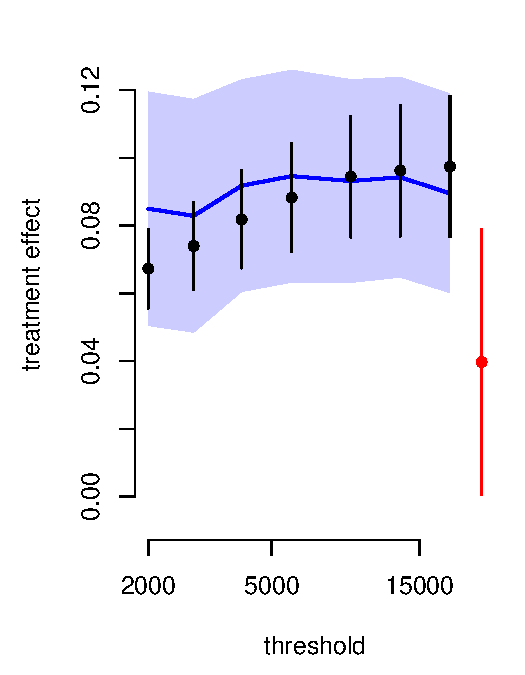
\includegraphics[width=.34\textwidth]{graphs/AB-tid32099.pdf}\!\!\!
%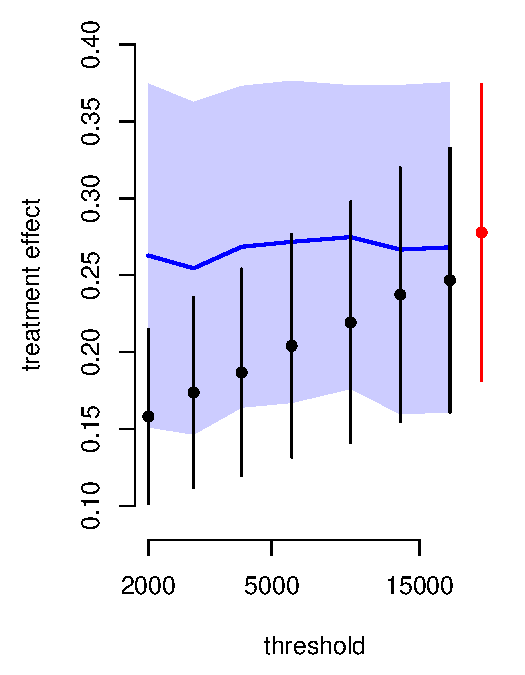
\includegraphics[width=.25\textwidth]{graphs/AB-tid32350.pdf}\!\!
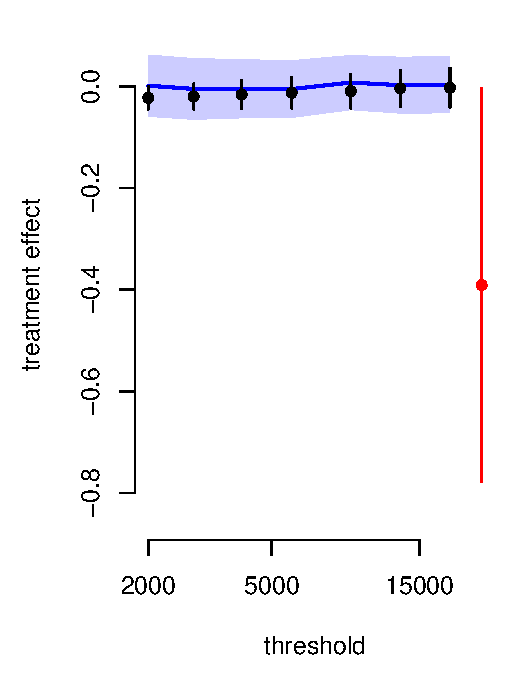
\includegraphics[width=.34\textwidth]{graphs/AB-tid33444.pdf}\!\!\!
\end{center}

\vskip -.25cm
Such care in uncertainty quantification is essential whenever you need to understand the full posterior (or sampling) distribution. {\gr e.g., bandit learning with heavy-tailed rewards is another application.\!\!\!}
\vskip -.25cm
\end{frame}

\begin{frame}

\vskip .5cm
{\bf Big Data and distribution-free BNP}

\vskip .25cm I think about BNP as a way to analyze (and improve) algorithms.  

Decouple action/prediction from the full generative process model.

\vskip .25cm  This type of analysis is key for taking these algorithms from ML \\to fields like Economics that really care about uncertainty.

\vskip .75cm
{\bf Efficient Big Data analysis}

\vskip .25cm
To cut computation without hurting performance, we need to think about what portions of the `model' are {\theme hard} or {\nv easy} to learn.

\vskip .25cm
Once we figure this out,  we can use a little bit of the data to\\ learn the easy stuff and direct our full data at the hard stuff.

\vskip .25cm
This is {\it the} future for Big Data.

\hfill \huge \theme \bf thanks!

\end{frame}



\end{document}






























